\subsection{Runge's Theorem}
By definition, a rational function is the quotient of two polynomials; and by \cref{thm:rationalmeromorphicfunctions}, in equivalent formulation, it is a function meromorphic on all of \(\extcomplex\). The poles and zeros may not accumulate in \(\extcomplex\), and thus there are finitely many as a consequence of Bolzano--Weierstrass (\cref{thm:bolzanoweierstrass}).

When we refer to approximation, we refer to the approximation of a function as the uniform limit (of a sequence) of functions. Let \(K\subset\mathbb{C}\) be compact and suppose \(f:K\to\mathbb{C}\) is a given function on \(K\). As a consequence of Mergelyan's Theorem (\cref{thm:mergelyan}), sufficient conditions for \(f\) to be the uniform limit of rational functions whose poles lie in (a subset of given points of) \(\extcomplex\setminus K\) are the continuity of \(f\) on \(K\) and the holomorphy of \(f\) on \(\interior{K}\).

In the earliest formulation by Carl Runge in 1885, he provided the sufficiency of the holomorphy of \(f\) on \(K\) (in effect, a neighborhood of \(K\)).

The proof can be well-organized through the use of the results that we will now introduce. In essence, it involves applying Cauchy--Goursat to \(f\) and the subsequent use of Riemann sums to approximate the complex line integral.
\begin{proposition}\label{prop:rungesimplepolesandremovablesingularityatinfinity}
    Let \(K\subset\mathbb{C}\) be compact and suppose \(U\supset K\) is a neighborhood of \(K\) that is relatively compact in \(\mathbb{C}\). Let \(f:U\to\mathbb{C}\) be an arbitrary holomorphic function. Then for fixed \(\varepsilon>0\), there exists a rational function \(\psi(z)\) with only simple poles (all of which lie in \(\mathbb{C}\setminus K\)) such that \[\lim_{z\to\infty}\psi(z)=0,\qquad\sup_{z\in K}\abs{f(z)-\psi(z)}<\varepsilon.\]
\end{proposition}
\begin{proof}
    By assumption of relative compactness, \(\mathrm{dist}(\partial U,\partial K)\), or the distance (infimum) between \(K\) and \(\mathbb{C}\setminus U\), is positive and finite. More concretely, let \[d=\inf\cbraces{\abs{z_1-z_2}}{z_1\in K,z_2\in\mathbb{C}\setminus U}>0\]
    The longest distance between two points in any square is the length of the diagonal. Hence, any square \(Q\) that intersects \(\partial K\) with a side length less than \(\frac{\sigma\sqrt{2}}{2}\) will lie completely within \(U\).

    \begin{figure}
        \centering
        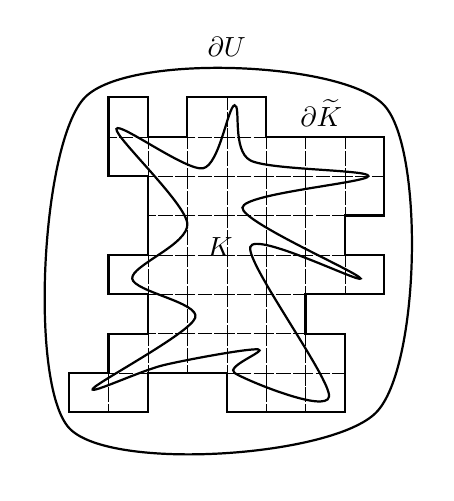
\begin{tikzpicture}
            \foreach \x in {0,...,7}
            \foreach \y in {0,...,7} {
                    \ifnum\x=0
                        \ifnum\y=1\else
                            \ifnum\y=2\else
                                \ifnum\y=3\else
                                    \ifnum\y=4\else
                                        \ifnum\y=5\else
                                            \ifnum\y=6\else
                                                \ifnum\y=7\else\draw[ultra thin, dashed] (0.5*\x,0.5*\y) rectangle ++(0.5,0.5);
                                                \fi\fi\fi\fi\fi\fi\fi \else
                        \ifnum\x=1
                            \ifnum\y=2\else
                                \ifnum\y=4\else
                                    \ifnum\y=5\else\draw[ultra thin, dashed] (0.5*\x,0.5*\y) rectangle ++(0.5,0.5);
                                    \fi\fi\fi \else
                            \ifnum\x=2
                                \ifnum\y=0\else
                                    \ifnum\y=7\else\draw[ultra thin, dashed] (0.5*\x,0.5*\y) rectangle ++(0.5,0.5);
                                    \fi\fi \else
                                \ifnum\x=3
                                    \ifnum\y=0\else\draw[ultra thin, dashed] (0.5*\x,0.5*\y) rectangle ++(0.5,0.5);
                                    \fi\else
                                    \ifnum\x=5
                                        \ifnum\y=7\else\draw[ultra thin, dashed] (0.5*\x,0.5*\y) rectangle ++(0.5,0.5);
                                        \fi\else
                                        \ifnum\x=6
                                            \ifnum\y=2\else
                                                \ifnum\y=7\else\draw[ultra thin, dashed] (0.5*\x,0.5*\y) rectangle ++(0.5,0.5);
                                                \fi\fi\else
                                            \ifnum\x=7
                                                \ifnum\y=0\else
                                                    \ifnum\y=1\else
                                                        \ifnum\y=2\else
                                                            \ifnum\y=4\else
                                                                \ifnum\y=7\else\draw[ultra thin, dashed] (0.5*\x,0.5*\y) rectangle ++(0.5,0.5);
                                                                \fi\fi\fi\fi\fi\else
                                                \draw[ultra thin, dashed] (0.5*\x,0.5*\y) rectangle ++(0.5,0.5);
                                            \fi\fi\fi\fi\fi\fi\fi
                }
            \draw[thick] (0,0) -- (0,0.5) -- (0.5,0.5) -- (0.5,1) -- (1,1) -- (1,1.5) -- (0.5,1.5) -- (0.5,2) -- (1,2) -- (1,3) -- (0.5,3) -- (0.5,4) -- (1,4) -- (1,3.5) -- (1.5,3.5) -- (1.5,4) -- (2.5,4) -- (2.5,3.5) -- (4,3.5)-- (4,2.5) -- (3.5,2.5) -- (3.5,2) -- (4,2) -- (4,1.5) -- (3,1.5) -- (3,1) -- (3.5,1) -- (3.5,0) -- (2,0) -- (2,0.5) -- (1,0.5) -- (1,0) -- cycle;
            \draw[thick] plot[smooth cycle] coordinates {
                    (3.8,3) (2.2,2.6) (3.7,1.7) (2.3,2.1) (3.3,0.2) (2.1,0.5) (2.4,0.8) (1.2,0.6) (0.3,0.3) (1.6,1.2) (0.8,1.7) (1.5,2.4) (0.6,3.6) (1.7,3.1) (2.1,3.9) (2.3,3.2)
                };
            \draw[thick] plot[smooth cycle] coordinates {
                    (0,-0.2) (0.2,4) (4,3.9) (3.9,0)
                };
            \node[anchor=east] at (2.2,2.1) {\(K\)};
            \node[anchor=north] at (3.2,4.1) {\(\partial\widetilde{K}\)};
            \node[anchor=south] at (2,4.4) {\(\partial U\)};
        \end{tikzpicture}
        \caption{The elements of \(\mathcal{G}\), relative to \(K\) and its neighborhood, \(U\).}\label{fig:rungesimplepolesandremovablesingularityatinfinity_grid}
    \end{figure}Choose \(m\in\mathbb{N}\) to satisfy \(2^{1-m}<\sigma\) and consider the grid generated by compact squares in the form of \[\cbraces{x+\ii y}{\frac{j}{2^m}\leq x\leq\frac{j+1}{2^m},\frac{k}{2^m}\leq y\leq \frac{k+1}{2^m}}\] (where \(j\) and \(k\) are integers) and let \(\mathcal{G}\) be the collection of all such squares in this grid that intersect \(K\), and it follows that \(\widetilde{K}=\bigcup_{Q\in\mathcal{G}} Q\subset U\) (refer to \cref{fig:rungesimplepolesandremovablesingularityatinfinity_grid}).

    As a consequence of Cauchy--Goursat (\cref{thm:cauchygoursatformula}), we have
    \begin{equation}
        \frac{1}{2\uppi\ii}\oint_{\partial\widetilde{K}}\frac{f(\zeta)\ddzeta}{\zeta-z}=f(z)\label{eq:rungesimplepolesandremovablesingularityatinfinity_cauchygoursat}
    \end{equation} in the case that \(z\in\widetilde{K}\). The boundary \(\partial\widetilde{K}\) may be written as the union of \(n\) lines parameterized by \(0\leq t\leq 1\); more concretely, we have \(\partial\widetilde{K}=\bigcup_{j\in\mathbb{N}_{\leq n}}\gamma_j([0,1])\). Hence we have in equivalent formulation, \[f(z)=\frac{1}{2\uppi\ii}\sum_{j=1}^n\int_{\gamma_j([0,1])}\frac{f(\zeta)}{\zeta-z}\ddzeta=\frac{1}{2\uppi\ii}\sum_{j=1}^n\int_0^1\frac{f\qty(\gamma_j(t))\gamma'_j(t)}{\gamma_j(t)-z}\ddt.\]
    The distance between \(K\) and \(\partial\widetilde{K}\) is strictly positive. Suppose instead that the distance were zero. Then some point of \(K\) would lie on the boundary of a square \(Q\in\mathcal{G}\) that intersects \(\partial\widetilde{K}\). If this point lies on an edge of \(Q\) (but not at a vertex), then the square adjacent along that edge must also intersect \(K\), and hence belong to \(\mathcal{G}\), contradicting the assumption that the point lies on \(\partial\widetilde{K}\). If the point lies at a vertex of \(Q\), then all three adjacent squares also intersect \(K\), so they too belong to \(\mathcal{G}\), leading to the same contradiction. Thus, the distance must be positive.

    Hence, each integrand as defined in \cref{eq:rungesimplepolesandremovablesingularityatinfinity_cauchygoursat} is jointly continuous for \(t\in[0,1]\) and \(z\in K\). By compactness of the product, it is in fact uniformly continuous by Heine--Cantor (\cref{thm:heinecantor}).

    Hence, \(\forall\varepsilon>0\), \(\exists\delta>0\) such that \(\forall z\in K\), \(\forall 1\leq j\leq n\) (uniform in \(j\) as we can take the minimum of each \(\delta_j\)), and \(\forall t_1,t_2\in [0,1]\) satisfying \(\abs{t_1-t_2}<\delta\), \[\abs{\frac{f\qty(\gamma_j\qty(t_1))\gamma'_j\qty(t_1)}{\gamma_j\qty(t_1)-z}-\frac{f\qty(\gamma_j\qty(t_2))\gamma'_j\qty(t_2)}{\gamma_j\qty(t_2)-z}}<\frac{\varepsilon}{n}.\]
    Partition \([0,1]\) by \(0=t_0<t_1<\cdots<t_m=1\) such that \(\forall 0\leq k<m\), \(\Delta t_k=t_{k+1}-t_k<\delta\). It follows that
    \begin{multline*}
        \abs{f(z)-\frac{1}{2\uppi\ii}\sum_{j=1}^n\sum_{k=0}^{m-1}\frac{f\qty(\gamma_j\qty(t_k))\gamma'_j\qty(t_k)}{\gamma_j\qty(t_k)-z}\Delta t_k}\\
        =\frac{1}{2\uppi}\abs{\sum_{j=1}^n\sum_{k=0}^{m-1}\int_{t_k}^{t_{k+1}}\qty[\frac{f\qty(\gamma_j\qty(t))\gamma'_j\qty(t)}{\gamma_j\qty(t)-z}-\frac{f\qty(\gamma_j\qty(t_k))\gamma'_j\qty(t_k)}{\gamma_j\qty(t_k)-z}]\ddt}\\
        \leq\frac{1}{2\uppi}\sum_{j=1}^n\sum_{k=0}^{m-1}\int_{t_k}^{t_{k+1}}\abs{\frac{f\qty(\gamma_j\qty(t))\gamma'_j\qty(t)}{\gamma_j\qty(t)-z}-\frac{f\qty(\gamma_j\qty(t_k))\gamma'_j\qty(t_k)}{\gamma_j\qty(t_k)-z}}\ddt\\
        \leq\frac{\varepsilon}{2n\uppi}\sum_{j=1}^n\sum_{k=0}^{m-1}\Delta t_k=\frac{\varepsilon}{2\uppi}<\varepsilon
    \end{multline*} uniformly in \(z\in K\). The summation \[\psi(z)=\frac{1}{2\uppi\ii}\sum_{j=1}^n\sum_{k=0}^{m-1}\frac{f\qty(\gamma_j\qty(t_k))\gamma'_j\qty(t_k)}{\gamma_j\qty(t_k)-z}\Delta t_k\] defines a rational function with simple poles at each \(\gamma_j\qty(t_k)\in\partial\widetilde{K}\), which is disjoint from \(K\).
\end{proof}
In its full generality, we will now apply a technique to \emph{push} a pole to a prescribed point, while ensuring that the resulting function remains uniformly approximated outside of a given connected compact set that contains both the original and target pole locations.
\begin{lemma}[Pole-Pushing Lemma]\label{lem:simplepolepushing}
    Let \(\alpha,\beta\in\mathbb{C}\) and let \(f(z)\) be a rational function with a single singularity, a pole at \(z=\alpha\), whose Laurent expansion consists solely of its principal part. Then \(\forall r>\abs{\alpha-\beta}\), \(\forall\varepsilon>0\), there exists a rational function \(\psi(z)\) whose only singularity is a pole at \(z=\beta\) such that \[\sup_{z\in\extcomplex\setminus D(\beta,r)}\abs{f(z)-\psi(z)}<\varepsilon.\]
\end{lemma}
\begin{proof}
    By assumption, \(f\) can be expressed as a polynomial of
    \begin{align*}
        (z-\alpha)^{-1} & =(z-\beta)^{-1}\frac{1}{\qty(z-\alpha)\qty(z-\beta)^{-1}}=\qty(z-\beta)^{-1}\frac{1}{1-\qty(\alpha-\beta)(z-\beta)^{-1}} \\
                        & =\qty(z-\beta)^{-1}\sum_{k=0}^\infty\qty(\frac{\alpha-\beta}{z-\beta})^k.
    \end{align*}
    This series locally uniformly converges on \[\cbraces{z\in\extcomplex}{\abs{\alpha-\beta}\abs{z-\beta}^{-1}<1}=\extcomplex\setminus\overline{D\qty(\beta,\abs{\alpha-\beta})}\] and uniformly converges on \(\extcomplex\setminus D(\beta,r)\). Hence, for \(m\in\mathbb{N}\), we have \[f(z)=\sum_{j=1}^{m}a_{-j}\qty[\qty(z-\beta)^{-1}\sum_{k=0}^\infty\qty(\frac{\alpha-\beta}{z-\beta})^k]^j.\]
    For fixed \(j\) (where \(a_{-j}\neq 0\)), we aim to prove the existence of an \(N\in\mathbb{N}\) such that \(\forall n>N\), we have at least
    \begin{equation}
        \abs{\qty[(z-\beta)^{-1}\sum_{k=0}^\infty\qty(\frac{\alpha-\beta}{z-\beta})^k]^j-\qty[(z-\beta)^{-1}\sum_{k=0}^n\qty(\frac{\alpha-\beta}{z-\beta})^k]^j}<\frac{\varepsilon}{m\abs{a_{-j}}},\label{eq:simplepolepushing_uniformboundassumption}
    \end{equation} where \(z\in\extcomplex\setminus D(\beta,r)\). Since \(\abs{\frac{1}{z-\beta}}<\frac{1}{r}\), we can restrict \cref{eq:simplepolepushing_uniformboundassumption} further with \[\abs{\qty[\sum_{k=0}^\infty\qty(\frac{\alpha-\beta}{z-\beta})^k]^j-\qty[\sum_{k=0}^n\qty(\frac{\alpha-\beta}{z-\beta})^k]^j}<\frac{r^j\varepsilon}{m\abs{a_{-j}}}.\]
    Additionally, the difference on the left-hand side is also equal to
    \begin{equation}
        \abs{\qty(\sum_{k=n+1}^\infty\qty(\frac{\alpha-\beta}{z-\beta})^k)\qty(\sum_{l=0}^{j-1}\qty[\sum_{k=0}^n\qty(\frac{\alpha-\beta}{z-\beta})^k]^l\qty[\sum_{k=0}^\infty\qty(\frac{\alpha-\beta}{z-\beta})^k]^{j-l-1})}.\label{eq:simplepolepushing_uniformboundassumption2}
    \end{equation} For any \(n\in\mathbb{N}\), we have \[\abs{\sum_{k=0}^n\qty(\frac{\alpha-\beta}{z-\beta})^k}\leq\sum_{k=0}^n\abs{\frac{\alpha-\beta}{z-\beta}}^k\leq\sum_{k=0}^\infty\abs{\frac{\alpha-\beta}{r}}^k\leq\frac{1}{1-\abs{\frac{\alpha-\beta}{r}}}.\] Since the dominating sequence of partial sums are monotonically increasing, it follows that the sequence of partial sums is uniformly bounded by \[M=\frac{r}{r-\abs{\alpha-\beta}}\] on \(\extcomplex\setminus D(\beta,r)\). Thus, \cref{eq:simplepolepushing_uniformboundassumption2} is bounded by \(M^{j-1}j\abs{\sum_{k=n+1}^\infty\qty(\frac{\alpha-\beta}{z-\beta})^k}\), and we apply further restriction by setting this to be bounded by \(\frac{r^j\varepsilon}{m\abs{a_{-j}}}\). By uniform convergence, for any \(\varepsilon>0\), \(\exists N_j\in\mathbb{N}\) such that \(\forall n>N_j\), \[\abs{\sum_{k=n+1}^\infty\qty(\frac{\alpha-\beta}{z-\beta})^k}<\frac{r^j\varepsilon}{M^{j-1}jm\abs{a_{-j}}}.\] For \(n>N_j\), \cref{eq:simplepolepushing_uniformboundassumption} is satisfied, and \(\forall n>\max_{\substack{j=1\\a_{-j}\neq 0}}^m\qty(N_j)\), \(z\in\extcomplex\setminus D(\beta,r)\), we have
    \begin{align*}
        \abs{f(z)-\sum_{j=1}^ma_{-j}\qty[\frac{1}{z-\beta}\sum_{k=0}^n\qty(\frac{\alpha-\beta}{z-\beta})^k]^j} & \leq\sum_{\substack{j=1 \\a_{-j}\neq 0}}^m\abs{a_{-j}}\abs{\qty[\sum_{k=0}^\infty\qty(\frac{\alpha-\beta}{z-\beta})^k]^j-\qty[\sum_{k=0}^n\qty(\frac{\alpha-\beta}{z-\beta})^k]^j}\\
                                                                                                               & \leq\sum_{\substack{j=1 \\a_{-j}\neq 0}}^m\abs{a_{-j}}\frac{\varepsilon}{m\abs{a_{-j}}}\leq\varepsilon,
    \end{align*}
    which completes the proof as \[\psi(z)=\sum_{j=1}^ma_{-j}\qty[(z-\beta)^{-1}\sum_{k=0}^n\qty(\frac{\alpha-\beta}{z-\beta})^k]^j\] is rational with a pole at \(z=\beta\).
\end{proof}
\begin{lemma}[Generalized Pole-Pushing Lemma]\label{lem:generalpolepushing}
    Let \(K\subset\mathbb{C}\) be compact and choose \(a\in\mathbb{C}\setminus K\). Let \(U\) be the connected component of \(\extcomplex\setminus K\) containing \(a\). Then \(\forall\varepsilon>0\), \(\forall\zeta\in U\), there exists a rational function \(\psi\) with a pole only at \(\zeta\) such that \[\sup_{z\in K}\abs{\frac{1}{z-a}-\psi(z)}<\varepsilon.\]
\end{lemma}
\begin{proof}
    Define the set
    \[S=\cbraces{\zeta\in U\setminus\cbraces{\infty}}{(\forall\varepsilon>0)(\exists\psi)\qty[\bigwedge
                \begin{aligned}
                     & \psi\text{ is rational},                                                             \\
                     & \psi(\mathbb{C}\setminus\cbraces{\zeta})\subseteq\mathbb{C}\wedge\psi(\zeta)=\infty, \\
                     & \sup_{z\in K}\abs{\frac{1}{z-a}-\psi(z)}<\varepsilon
                \end{aligned}]}.\]
    Since \(a\in U\) satisfies the condition with \(\psi(z)=\frac{1}{z-a}\), it follows that \(a\in S\), ensuring that \(S\) is nonempty.

    Consider \(\zeta\in S\), where \(\zeta\) lies in the complement of \(K\). The distance from \(\zeta\) to \(K\), denoted \(\mathrm{dist}(\zeta,K)\), is positive, and the open disk \(D(\zeta,\mathrm{dist}(\zeta,K))\) is disjoint from \(K\). Let \(\zeta'\) be an arbitrary point in this disk. By the definition of \(S\), for every \(\varepsilon>0\), there exists a rational function \(\psi\) with a pole only at \(\zeta\) such that
    \[\sup_{z\in K}\abs{\frac{1}{z-a}-\psi(z)}<\frac{\varepsilon}{2}.\]
    By \cref{lem:simplepolepushing}, there exists a rational function \(\phi\) with a pole only at \(\zeta'\) such that
    \[\sup_{z\in\extcomplex\setminus D(\zeta,\mathrm{dist}(\zeta,K))}\abs{\phi(z)-\psi(z)}<\frac{\varepsilon}{2},\]
    which implies
    \[\sup_{z\in K}\abs{\phi(z)-\psi(z)}<\frac{\varepsilon}{2}.\]
    Thus,
    \[\sup_{z\in K}\abs{\frac{1}{z-a}-\phi(z)}\leq\sup_{z\in K}\abs{\frac{1}{z-a}-\psi(z)}+\sup_{z\in K}\abs{\psi(z)-\phi(z)}<\varepsilon,\]
    and by definition, \(\zeta'\in S\Rightarrow D\qty(\zeta,\mathrm{dist}\qty(\zeta,K))\subseteq S\). Hence, \(S\) is relatively open in \(U\setminus\cbraces{\infty}\).

    Now, consider \(\zeta\in U\setminus\qty(S\cup\cbraces{\infty})\). Suppose there exists \(\zeta'\in D(\zeta,\mathrm{dist}(\zeta,K))\cap S\). By repeated application of the preceding argument, this would imply \(\zeta\in S\), contradicting the assumption that \(\zeta\in U\setminus\qty(S\cup\cbraces{\infty})\). Therefore, no such \(\zeta'\) exists, and \(S\) is relatively closed in \(U\setminus\cbraces{\infty}\).

    Since \(U\setminus\cbraces{\infty}\) is connected and \(S\) is both relatively open and closed in \(U\setminus\cbraces{\infty}\), it follows from \cref{thm:connectedtopologicalspaceclopensets} that \(S=U\setminus\cbraces{\infty}\), completing the proof under the assumption that \(\infty\notin U\).

    Now suppose \(\infty\in U\). In essence, we pole push to a point outside a disk on which we can make approximations by Taylor polynomials. Let \(R>0\) satisfy \(K\subset D(0,R)\) and let \(b\in U\setminus\qty(\cbraces{\infty}\cup\overline{D(0,R)})\) be an arbitrary point. By \cref{lem:simplepolepushing}, there exists some rational function \(\widetilde{\psi}(z)\) with a pole at \(b\) such that \[\sup_{z\in K}\abs{\widetilde{\psi}(z)-\frac{1}{z-a}}<\frac\varepsilon2.\]
    Since \(\widetilde{\psi}\) is holomorphic on some neighborhood of \(\overline{D(0,R)}\), we have \[\widetilde{\psi}(z)=\sum_{k=0}^\infty a_k z^k\qq{on}\overline{D(0,R)},\] and it uniformly converges on \(\overline{D(0,R)}\). Hence, \(\exists N\in\mathbb{N}\) such that \[\sup_{z\in\overline{D(0,R)}}\abs{\widetilde{\psi}(z)-\sum_{k=0}^N a_k z^k}<\frac{\varepsilon}{2}.\]
    Since polynomials have poles at \(\infty\), we have \[\sup_{z\in\overline{D(0,R)}}\abs{\frac{1}{z-a}-\sum_{k=0}^N a_k z^K}\leq\sup_{z\in\overline{D(0,R)}}\abs{\frac{1}{z-a}-\widetilde{\psi}(z)}+\sup_{z\in\overline{D(0,R)}}\abs{\widetilde{\psi}(z)-\sum_{k=0}^N a_kz^k}<\varepsilon.\qedhere\]
\end{proof}
\begin{theorem}[Runge]\label{thm:runge}
    Let \(K\subset\mathbb{C}\) be compact such that \(\extcomplex\setminus K\) has finitely many connected components and suppose \(f\) is holomorphic on a neighborhood of \(K\). Let \(E\) be a subset of \(\extcomplex\setminus K\) containing one point from each of its connected components. Then \(\forall\varepsilon>0\), there is a rational function \(\psi\) whose poles lie in \(E\) such that \[\sup_{z\in K}\abs{f(z)-\psi(z)}<\varepsilon.\]
\end{theorem}
\begin{proof}
    By \cref{prop:rungesimplepolesandremovablesingularityatinfinity}, there is a rational function \(\phi\) with simple poles in \(\mathbb{C}\setminus K\) satisfying \(\phi(\infty)=0\) such that
    \begin{equation}
        \sup_{z\in K}\abs{f(z)-\phi(z)}<\frac\varepsilon2.\label{eq:runge_intermediate1}
    \end{equation}
    Let the poles of \(\phi\) be \(\cbraces{\beta_k}_{k\in\mathbb{N}_{\leq n}}\subset\mathbb{C}\setminus K\), and as a consequence, we have \(\phi(z)=\sum_{k=1}^n\frac{a_k}{z-\beta_k}+\varphi(z)\) where \(\varphi(z)\) is entire. Since \(\phi(\infty)=0\), we have \(\varphi\equiv 0\) by Liouville's Theorem (\cref{thm:liouville}). By \cref{lem:generalpolepushing}, there exist rational functions \(\cbraces{\psi_k}_{k\in\mathbb{N}_{\leq n}}\) whose only poles lie in \(E\) such that \(\forall k\), \[\sup_{z\in K}\abs{\frac{1}{z-\beta_k}-\psi_k(z)}<\frac{\varepsilon}{2n\abs{a_k}}\] and it follows that \[\sup_{z\in K}\abs{\phi(z)-\sum_{k=1}^n a_k\psi_k(z)}\leq\sup_{z\in K}\sum_{k=1}^n\abs{\frac{a_k}{z-\beta_k}-a_k\psi_k(z)}<\frac\varepsilon2.\]
    Let \(\psi(z)=\sum_{k=1}^na_k\psi_k(z)\). From \cref{eq:runge_intermediate1}, we have \[\sup_{z\in K}\abs{f(z)-\psi(z)}\leq\sup_{z\in K}\abs{f(z)-\phi(z)}+\sup_{z\in K}\abs{\phi(z)-\psi(z)}<\varepsilon.\qedhere\]
\end{proof}
